\chapter{Proposed Methodology}

% Cambridge-driving Labeled Video Database (CamVid)
% Video Scene Parsing in the Wild (VSPW)
% Actor and Action (A2D)
% Densely Annotated VIdeo Segmentation(DAVIS)
% Multi-Object Tracking and Segmentation(MOTS)
% Berkeley DeepDrive (BDD)
% Video Object Segmentation(VOS)
% Video Instant Segmentation(VIS)
% Region-Based CNNs (R-CNN)
% Single Shot MultiBox Detector (SSD)
% Computer Vision and Pattern Recognition (CVPR)


\nomenclature{YOLO}{You Only Look Once}

\nomenclature{CamVid}{Cambridge-driving Labeled Video Database}

\nomenclature{VSPW}{Video Scene Parsing in the Wild}

\nomenclature{A2D}{Actor and Action}

\nomenclature{DAVIS}{Densely Annotated VIdeo Segmentation}

\nomenclature{MOTS}{Multi-Object Tracking and Segmentation}

\nomenclature{BDD}{Berkeley DeepDrive}

\nomenclature{FBMS}{Freiburg-Berkeley Motion Segmentation}

\nomenclature{VOS}{Video Object Segmentation}

\nomenclature{VIS}{Video Instant Segmentation}

\nomenclature{R-CNN}{Region-Based Convolutional Neural Networks}

\nomenclature{SSD}{Single Shot MultiBox Detector}

\nomenclature{CVPR}{Computer Vision and Pattern Recognition}

% ------------------------------------------------------------

\section{Introduction}

\begin{figure}[h]
    \centering
    
\includegraphics[width=\textwidth]{Images/high_level_overview_of_the_system.png}
    \caption{High-Level Overview of the System}
\end{figure}

\noindent
Figure 3.1 shows a high-level overview of the process of automatic segmentation and labeling of objects in videos. The steps involved are:
\\

\textbf{Step 1: Video Input}\\
The first step is to input the video sequence into the system. This can be done by loading the video file from a disk or by streaming the video from a live feed.\\
\\
\textbf{Step 2: Frame Identification}\\
Once the video input has been loaded, the system needs to identify the individual frames in the video sequence. This can be done by extracting each frame from the video file or by using a more sophisticated motion detection algorithm to identify the frames where there is significant motion.

\noindent
\textbf{Step 3: Object Segmentation and Labelling}\\
After the individual frames in the video have been identified, the system needs to segment the objects in each frame. This can be done using a variety of computer vision algorithms, such as Optical flow, Background subtraction, and Deep learning algorithms.\\
Then the system needs to label the objects. This can be done by using a variety of methods, such as Rule-based labeling, Machine learning, Human-in-the-loop labeling, etc.

\begin{figure}[h]
    \centering
    
\includegraphics[width=\textwidth]{Images/Block_Diagram.png}
    \caption{Block Diagram of the Proposed System}
\end{figure}

\begin{enumerate}
    \item \textbf{Video Input:}

    The Video Input block serves as the system's entry point, accepting a continuous stream of video data. The video input is the raw material that undergoes subsequent processing stages to extract meaningful information and insights.

    % This stream can originate from various sources such as surveillance cameras, video files, or live broadcasts. 
    
     \item \textbf{Frame Interpolation Algorithm:}
     
     The Frame Interpolation Algorithm plays a crucial role in enhancing the temporal resolution of the video. By generating additional frames between existing ones, this algorithm smoothens motion transitions, resulting in a visually improved video. Techniques like optical flow analysis and interpolation methods are often employed to achieve this, contributing to a more seamless viewing experience.\\

     \item\textbf{Frame by Frame Splitting}

     In the "Frame by Frame Splitting" stage, the continuous video stream is segmented into individual frames. Each frame is treated as an independent image, enabling detailed analysis and processing. This step sets the foundation for subsequent feature extraction and object recognition processes, as it allows the system to focus on individual frames for precise examination.
     
     \item\textbf{CNN:}

     The CNN involves the application of Convolutional Neural Networks, a type of deep learning model designed for image-related tasks. In this context, the CNN extracts high-level features from each frame. These features may include edges, textures, and patterns that are crucial for understanding the content of the video. The CNN serves as a powerful tool for object recognition and scene understanding.
     
     \item\textbf{Identifying Objects in Frame:}

     The "Identifying Objects in Frame" block employs an object detection algorithm to recognize and locate objects within each frame. This algorithm leverages the features extracted by the CNN to make predictions about the presence and position of objects. Common techniques for object detection include Region-Based CNNs (R-CNN), You Only Look Once (YOLO), and Single Shot MultiBox Detector (SSD).In this method, YOLO V8 was used.
     
     \item\textbf{Separate Different Objects:}

     Following object identification, this stage involves a process to isolate and distinguish individual objects from one another within a frame. This separation is crucial for tracking and analyzing each object independently throughout the video sequence. Techniques like clustering or bounding box analysis may be employed to achieve this separation.

     \clearpage
     
     \item\textbf{Semantic/Instance Segmentation:}

     This block focuses on understanding the content of each frame at a pixel level. Semantic segmentation classifies each pixel into a specific class (e.g., person, car, background), while instance segmentation goes further by distinguishing between individual instances of the same class. This detailed segmentation provides a richer representation of the scene.
     
     \item\textbf{Labeling:}

     In this stage, labels are assigned to segmented regions, providing a descriptive identification of the content. These labels convey information about the category or class of each object or region within the frame. The labeling step enhances the interpretability of the video data and facilitates subsequent analysis.
     
     \item\textbf{Object Detection Algorithm:}

     The final "Object Detection Algorithm" block signifies another instance of object detection, possibly applied after segmentation and labeling. This step may involve a more refined analysis to detect objects that were not initially identified or to improve the accuracy of the previous detection results. It contributes to a comprehensive understanding of the video content, ensuring that no relevant objects are overlooked.  
    
\end{enumerate}

\noindent In summary, this block diagram outlines a sophisticated video processing pipeline, highlighting the significance of each stage in extracting valuable information and insights from the input video stream. The combination of frame interpolation, deep learning-based feature extraction, object detection, segmentation, labeling, and refined object detection results in a holistic approach to video analysis.

\clearpage

\section{Data Collection}

The method of Data Collection by harnessing camera-captured images and videos for training, rather than relying solely on large pre-annotated datasets, introduces a paradigm shift in the efficiency of segmentation and labeling processes. By leveraging real-world visual data captured by cameras, we not only tap into the richness and diversity of dynamic environments but also minimize the need for extensive manual annotation efforts. Utilizing these unlabeled or minimally labeled datasets allows for the development of more robust and adaptable models. Self-supervised learning techniques, such as leveraging temporal coherence and spatial context within videos, enable the algorithm to learn intrinsic patterns and relationships autonomously. This approach not only streamlines the training pipeline but also ensures that the model gains a nuanced understanding of the complexities present in real-world scenarios, ultimately enhancing the generalization and real-world applicability of automated segmentation and labeling systems. Due to its lack of scalability, Large datasets can be used which are as follows:

\begin{itemize}
\item \textbf{YouTube-Objects Dataset:} It comprises videos sourced from YouTube by searching for the names of 10 object categories from the PASCAL VOC Challenge. It includes 9 to 24 videos per class, with each video lasting between 30 seconds and 3 minutes. The videos have weak annotations, ensuring that each one contains at least one object related to its respective class.

\item \textbf{Freiburg-Berkeley motion segmentation (FBMS):} The dataset is a comprehensive benchmark consisting of 59 sequences. It provides precise ground truth annotations for moving objects at the pixel level.

\item \textbf{Davis16:} A benchmark dataset for object tracking and segmentation in computer vision. It comprises 50 video sequences with challenging conditions like occlusions and appearance changes. Each frame has pixel-level annotations for the main object.

\clearpage

\item \textbf{Davis17:} It expands on Davis16, offering 150 video sequences with varied challenges for object tracking and segmentation algorithms. It maintains high-quality annotations for evaluating algorithms in real-world complex scenarios.

\noindent
The community that holds DAVIS datasets runs an annual committee competition of Video Object Segmentation(VOS) and Video Instant Segmentation(VIS) in the DAVIS dataset.


\item \textbf{YouTube-VOS:} A benchmark dataset and challenge designed for advancing the field of video segmentation in computer vision. Introduced by Google Research, YouTube-VOS comprises high-resolution video sequences with pixel-level annotations for object segmentation. This dataset is a vital resource for evaluating and benchmarking the performance of algorithms in the challenging task of segmenting objects across consecutive video frames. 


\item \textbf{A2D Sentence:} A2D, or "Actions in the Datasets," is a dataset specifically curated for action recognition in video sequences. This dataset provides a diverse collection of video clips capturing a wide range of human actions in various everyday scenarios. A2D is instrumental in training and evaluating algorithms designed for action recognition, enabling researchers and practitioners to enhance the performance of computer vision models. The dataset's rich content and labeled annotations contribute significantly to the development of robust systems capable of understanding and interpreting human actions in dynamic video environments.

\item \textbf{CamVid:} Short for Cambridge-driving Labeled Video Database, is a widely used dataset in the field of computer vision and semantic segmentation. Created by the University of Cambridge, CamVid consists of high-resolution video sequences recorded from the perspective of a driving car. The dataset is annotated, providing pixel-level labels for various semantic classes such as road, building, pedestrian, and car. It is a valuable resource for training and evaluating algorithms in the challenging task of semantic segmentation, particularly in urban driving scenarios.

\clearpage

\item \textbf{VSPW:} VSPW stands for Video Scene Parsing in the Wild. It is a large-scale dataset for video scene parsing that was introduced in the 2021 paper "VSPW: A Large-scale Dataset for Video Scene Parsing in the Wild"\cite{VSPW_paper}. The VSPW dataset is annotated with pixel-level semantic labels for each frame. The labels are organized into 29 categories, including objects, such as cars, people, and trees; and scene categories, such as roads, sidewalks, and sky.

% \clearpage

\item \textbf{MOTSChallenge:} The Multiple Object Tracking and Segmentation (MOTS) Challenge is an annual competition that evaluates the performance of state-of-the-art algorithms for tracking and segmenting multiple objects in videos. The challenge is organized by the Multi-Object Tracking Benchmarking Taskforce (MOTChallenge) and is held in conjunction with the Conference on Computer Vision and Pattern Recognition (CVPR). 

\item \textbf{BDD100K:} BDD100K is a large-scale driving video dataset that was released in 2018. It is the largest and most diverse open-driving video dataset to date, with over 100,000 videos and 10 tasks. The dataset was collected by Nexar, a company that develops dashcams for cars. The videos were collected in a variety of cities around the world, including San Francisco, Los Angeles, and New York City. 
\end{itemize}

\noindent
See Table 3.1 for short summary of the datasets explained above.\\

\noindent
Overall, the process of automatic segmentation and labeling of objects in video represents a transformative leap in the realm of computer vision, offering unparalleled efficiency and scalability. The collection of data for this purpose is a cornerstone in training robust machine learning models. By automating the segmentation and labeling tasks, we alleviate the burden of manual annotation, which is not only time-consuming but also prone to human errors. The datasets curated for automatic segmentation and labeling serve as invaluable resources, capturing the diversity and complexity of real-world scenarios.

\clearpage

\begin{table}[htbp]
\centering
\resizebox{\textwidth}{!}{%
\begin{tabular}{|>{\centering\arraybackslash}p{3.2cm}|p{1cm}|p{10cm}|}
\hline
\multicolumn{1}{|c|}{\textbf{Dataset}} & \multicolumn{1}{|c|}{\textbf{Year}} & \multicolumn{1}{|c|}{\textbf{Description}} \\ \hline
CamVid & 2009 & 4 videos with pixel-level annotations for 32 object classes. \\ \hline
YouTube-Objects & 2012 & 1,407 videos with object-level annotations for 10 object classes. \\ \hline
FBMS & 2014 & 59 videos with object-level annotations for 10 object classes. \\ \hline
DAVIS16 & 2016 & 50 videos with object-level annotations for 30 object classes. \\ \hline
DAVIS17 & 2017 & 150 videos with instance-level annotations for 30 object classes. \\ \hline
YouTube-VOS & 2018 & 4,519 videos with pixel-level annotations for 65 object classes. \\ \hline
A2D Sentence & 2018 & 3,782 videos with annotations for referring to objects in natural language. \\ \hline
MOTSChallenge & 2019 & 4 sequences of images from surveillance cameras with annotations for 2D tracking of vehicles and pedestrians. \\ \hline
BDD100K & 2020 & 1 Lakh driving scenes images with pixel-level annotations for 8 object classes. \\ \hline
VSPW & 2021 & 3,536 videos with pixel-level annotations for 8 object classes. \\ \hline
\end{tabular}%
}
\caption{Summary of Datasets with Annotations}
\end{table}

\noindent
The significance of data collection lies in shaping algorithms for autonomous systems, surveillance, and various applications. Labeled datasets enable accurate interpretation of visual information, aiding machines in navigating and interacting seamlessly. Moreover, datasets for segmentation and labeling drive advancements in real-time applications. Swift object identification for autonomous vehicles and anomaly detection in surveillance videos enhance system responsiveness. Collected data forms the foundation for intelligent, adaptive systems in complex environments.

% ----------------------------------------------------------------------

\section{Work Done So Far}

\nomenclature{SAM}{Segment Anything Model}

% \setcounter{equation}{0}

This chapter deals with the results and inferences derived from the work done for phase 1 of this project. It includes the procedure and result of automatic image segmentation and labeling (via detection).

\noindent
Before the main work of automatic video segmentation and labeling, work was done on automatic image segmentation and labeling using the Segment Anything (SAM) model for Image Segmentation and You Only Look Once for Object Detection. Figure 4.1 is the input image that is fed into the combination of Object Segmentation Detection Models. Figure 4.2 is the output after segmentation and detection.

\begin{figure}[h]
    \centering
    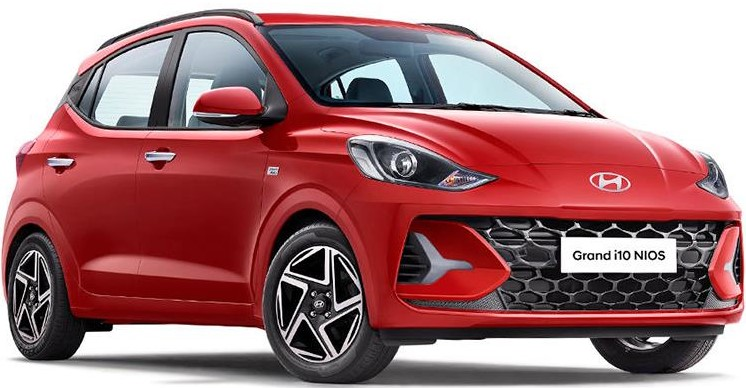
\includegraphics[width=0.6\textwidth]{Images/car.jpg}
    \caption{Input for Automatic Image Segmentation and Labeling}
\end{figure}

\clearpage

\begin{figure}[h]
    \centering
    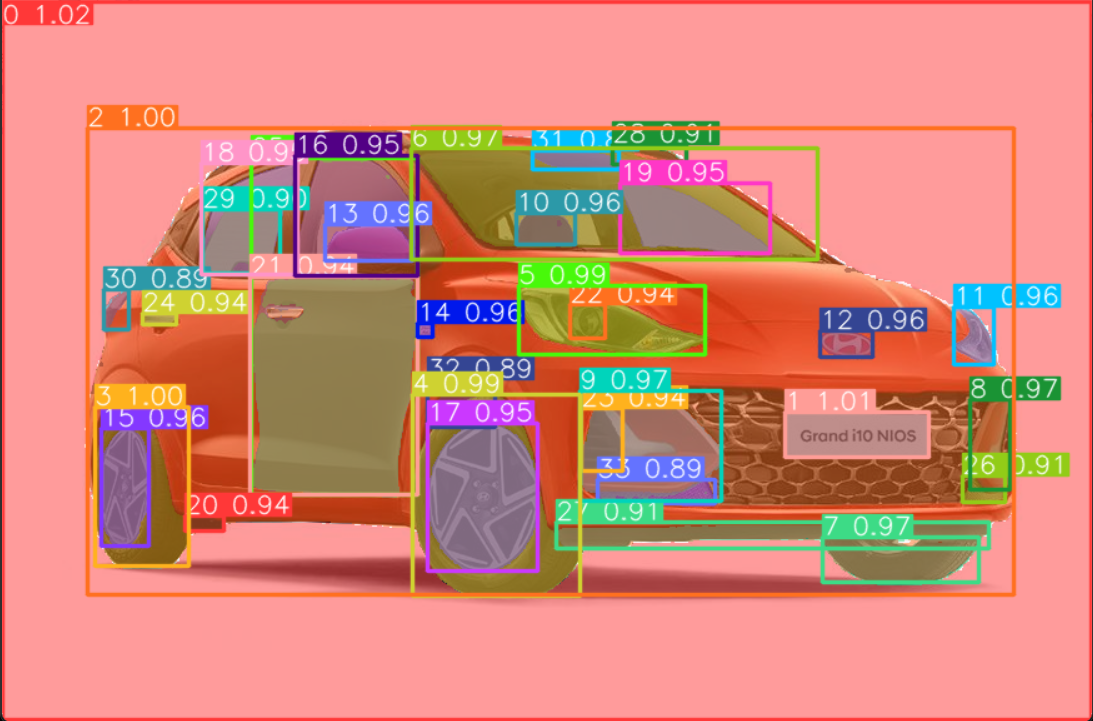
\includegraphics[width=.7\textwidth]{Images/car_sam_yolo.png}
    \caption{Output from Automatic Image Segmentation and Labeling}
\end{figure}

\noindent
When an image is inputted to a segmentation and object detection model together, the segmentation model focuses on dividing the image into distinct segments or regions based on pixel-level classification. This means it assigns a label to each pixel, outlining the boundaries and identifying areas belonging to different objects or categories within the image. On the other hand, the object detection model detects and localizes specific objects within the image. It identifies bounding boxes around these objects and assigns them labels, indicating the class or category of each object detected.

\noindent
The results from Figure 4.2 can be divided into two parts, segmentation and object labeling. The segmentation has worked well as the SAM Model is trained on tens of thousands of wide variety data, but the detection using YOLOv8 is not that accurate as the model is trained on some general classes like person, bicycle, car, bus, etc... but not specific parts of a car( as per figure 4.1) like door, mirror, and light. 